\chapter{Análisis y diseño}
\label{chap:analisis-disenho}


\lettrine{E}{n} este capítulo nos centraremos en el análisis y posterior diseño realizado en este \acrshort{tfg}.

\section{Análisis de las necesidades}
\label{sec:analisis}
Se pretende desarrollar una aplicación web que permita registrar las distintas contrataciones realizadas por los clientes de una empresa proveedora de servicios. Puesto que las contrataciones se realizan sobre el catálogo de servicios de la empresa, también proveerá de las herramientas necesarias para mantener dicho catálogo. Asimismo deberá permitir definir una serie de elementos parmetrizables necesarios para definir las distintas entidades que alberga dicha aplicación. Por lo tanto las entidades a tratar en el sistema se englobarán en tres grandes grupos:


\begin{itemize}
\item Parametrización: esta categoría engloba todos los elementos de parametrización necesarios para la definición de las distintas entidades del sistema (niveles de aplicación, tipos de descuento, tipos impositivos, etc.).
\item Catálogo: esta categoría engloba todos los elementos de que definen el catálogo de servicios la empresa (tipos de productos, servicios, cuotas, etc. y sus relaciones), así como los tipos de entidades que definen el catálogo de clientes y contrataciones (tipos de clientes, tipos de ciclos de facturación, etc.).
\item Instancia: esta categoría engloba todos los elementos que conforman las contrataciones: clientes, cuentas, elementos contratados, etc.
\end{itemize}


Dicha aplicación podrá ser utilizada por el personal del departamento de contratación y ventas de una empresa, que podrá llevar a cabo altas, bajas y modificaciones, así como personal de otros departamentos que puedan necesitar acceder a la información de la herramienta desarrollada con el fin de poder llevar a cabo sus tareas. Estos usuarios pertenecientes a otros departamentes han de tener limitado el acceso a las funcionalidades definidas en la aplicación. Además existirá una figura de administrador, que tendrá acceso a funcionalidades avanzadas.


Es por ello que se definen tres perfiles de acceso a la herramienta en función de las funcionalidades a las que se le quiera dar acceso al usuario. Dichos perfile serán los siguientes:

\begin{itemize}
\item READ: perfil que da sólo acceso a la consulta de los datos almacenados en el sistema, esto es, los usuarios que tengan este perfil asociado solo podrán listar la información, pero no podrán realizar ninguna modificación sobre los mismos.
\item WRITE: perfil que además de permitir la consulta de los datos almacenados en el sistema permite realizar altas, bajas y modificaciones sobre todos los elementos que conforman el sistema.
\item ADMIN: perfil que amplía el acceso a las funcionalidades definidas para el perfil WRITE, otorgándole acceso a la gestión de usuarios: podrá dar de alta nuevos usuarios, modificar usuarios existentes (incluido el cambio de contraseña) o darlos de baja.
\end{itemize}


Con el fin de poder hacer un seguimiento de los distintos cambios producidos en el sistema se deberá llevar registro de la creación de los elementos  del catálogo y de las instancias, así como de la última modificación realizada.

También con el objetivo de poder llevar un registro sobre los cambios producidos sobre determinadas entidades que pueden sufrir cambios durante su ciclo de vida se establecen registros de histórico para dichas entidades. El objetivo de estos históricos es poder tener la \textit{foto} del estado de una determinada entidad en un momento determinado, por ejemplo, el precio que tenía la definición de una cuota determinada o los distintos servicios activos de un cliente en una fecha determinada.


Esta aplicación tendrá el objetivo de formar parte de un ecosistema mayor, integrándose en una segunda fase con el resto de herramientas de la empresa para conformar el área comercial de la misma (figura \ref{fig:area-comercial}, \pageref{fig:area-comercial})

\begin{figure}[hp!]
  \centering
  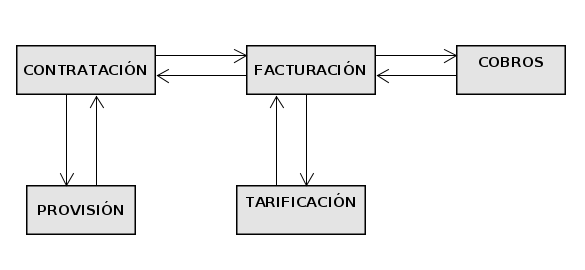
\includegraphics[width=0.50\textwidth]{imaxes/area-comercial.png}
  \caption{Entorno comercial}
  \label{fig:area-comercial}
\end{figure}


\subsection{Catálogo de servicios}
\label{sub:catalogo}

\acrshort{itil} define el catálogo de servicios como~\cite{catalogoITIL}:
\textquote{una base de datos centralizada que contiene información precisa sobre las ofertas de servicios de TI activas y un subconjunto de la cartera de servicios del proveedor de servicios de TI}. De forma simple vendría siendo la \textit{mercancía} que ofrece una determinada empresa. Pero va un paso más allá del listado de elementos ofertados en este momento, si no que  lleva registro del ciclo de vida de todos los productos y servicios gestionados por la empresa, tanto los servicios y productos retirados como los que se ofrecen actualmente e incluso los que están en desarrollo.

La idea es la siguiente: la empresa define su catálogo de servicios(tecnología a ofertar), los elementos facturables a aplicar por la prestación de servicios y los descuentos existentes sobre dichos elementos facturables. Se distinguen dos tipos de elementos facturables: cuotas (cargos periódicos asociados a la prestación de los distintos servicios) y consumos (cargos puntuales derivados del consumo de algún elemento definido como consumible)
El catálogo de servicio de nuestra empresa estará formado por cinco entidades principales y las relaciones que guardan entre sí (figura \ref{fig:catalogo}, página \pageref{fig:catalogo}):

\paragraph{Tipo de producto} es el elemento raiz del catálogo del sistema sobre el que se irán definiendo el resto de elementos que se pueden ofrecer al cliente. Podemos verlo como el \textit{paquete} que contendrá todo lo que se le ofrece al cliente.
\paragraph{Tipo de servicio} es el elemento que realmente aporta valor al cliente, ya que es el que define el elemento que va a aportar el valor de la contratación, por ejemplo la línea de telefono.
\paragraph{Tipo de promoción} es el elemento que definen los descuentos que define la empresa. Su ámbito de aplicación se circunscribe a productos y servicios y forma parte de su definición. El descuento se aplicará sobre los distintos elementos facturables existente en el sistema.
\paragraph{Tipo de cuota} es el elemento que define la contraprestación económica que va a recibir la empresa de forma periódica por la prestación de servicios que ofrece al cliente y su ámbito de aplicación se circunscribe a productos y servicios y forma parte de la definición del tipo de producto o servicio.
\paragraph{Tipo de consumos} es el elemento que define el consumo puntual de un determinado elemento por parte del cliente, como puede ser una llamada de teléfono. Sólo tiene interés desde el punto de vista de la definición de la aplicación de los distintos descuentos, ya que a diferencia de las cuotas, para las que podemos definir un precio cerrado que puede conocerse de antemano, el importe de los consumos vendrá definido por la naturaleza propia del evento del consumo (por ejemplo, el coste de una llamada de teléfono viene dada, además de por el tipo de llamada que lleva asociado un precio por minuto, por la duración de la misma o la franja horaria en la que se realiza) por lo que en la herramienta simplemente se definirán los consumos susceptibles de ser descontados. Se considera un único ámbito de aplicación: el de servicio.



\begin{figure}[hp!]
  \centering
  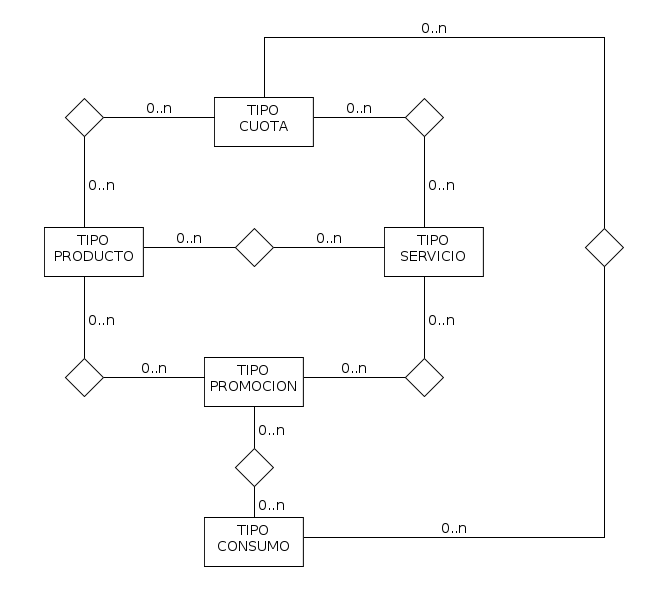
\includegraphics[width=0.50\textwidth]{imaxes/catalogo.png}
  \caption{Catálogo de servicios}
  \label{fig:catalogo}
\end{figure}


Puesto que el catálogo de servicios contiene la definición de los distintos elementos que podrán contratarse, hemos incluido dentro del concepto de catálogo otros elementos que permiten definir la plantilla con la que crear la posterior \textit{instanciación} de las mismas, a saber:

\paragraph{Tipo de ciclo de facturación} la instanciación de los distintos ciclos de facturación no forma parte del ámbito de la herramienta de contratación propiamente (entraría dentro del ámbito de facturación) pero puesto que forma parte de la definición de los distintos tipos de cuentas existentes, incluimos la definición del tipo de ciclo de facturación en la herramienta a desarrollar.

\paragraph{Tipo de cliente} esta entidad permitirá la creación de clientes atendiendo a una clasificación definida por la empresa, por ejemplo para distinguir entre clientes particulares de clientes de empresa.

\paragraph{Tipo de cuenta} la cuenta es la entidad sobre la que se realizarán las contrataciones, que a su vez dependerá de un cliente particular. La cuenta estará definida por una serie de valores especificados en la tipología de la misma, como el tipo de pago.



\subsection{Contratación}
\label{sub:contratacion}
La contratación contendrá la implementación (instancia) real de los distintos elementos definidos en el catálogo, esto es el conjunto de clientes y sus relaciones con los productos y servicios contratados (figura \ref{fig:contratacion}, \pageref{fig:contratacion}):



\begin{figure}[hp!]
  \centering
  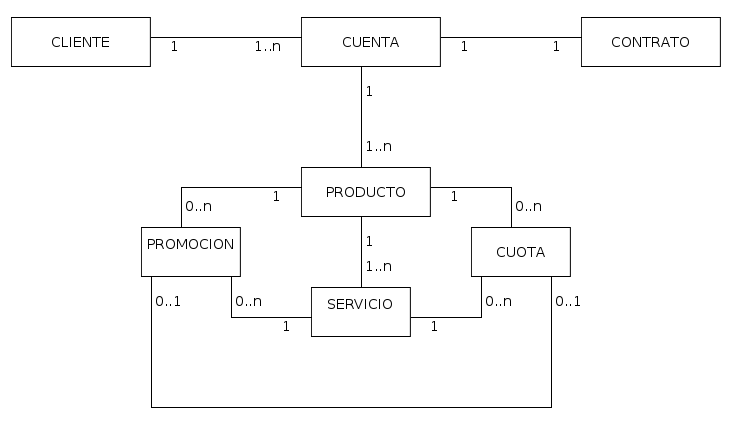
\includegraphics[width=0.50\textwidth]{imaxes/instancia.png}
  \caption{Contratación}
  \label{fig:contratacion}
\end{figure}


\subsection{Elementos de parametrización}
\label{sub:parametrizacion}
Los elementos de parametrización son elementos que nos permiten modelar entidades superiores para que se comporten de una forma determinada. No es lo mismo aplicar un descuento en forma de porcentaje sobre el total que en número de unidades contratadas. Para el desarrollo de la herramienta se han considerado los siguientes elementos de parametrización.

\paragraph{Entidades} define los distintos tipos de entidades definidas en el sistema.
\paragraph{Clases de consumo} define las distintas clases de consumo definidas en el sistema (llamadas a fijo, a móviles, sms,\dots).
\paragraph{Estado} para reflejar los distintos estados que tienen las entidades del sistema a lo largo de su ciclo de vida.
\paragraph{Nivel de aplicación} para indicar sobre qué entidad aplican las distintas cuotas y promociones: si sobre un producto o sobre un servicio.
\paragraph{Tipos de descuento} reflejan los distintos tipos de descuento que pueden tenerse en cuenta (porcentaje sobre el total, unidades de consumo,\dots).
\paragraph{Tipos de pago} reflejan los distintos métodos de pago que contempla la empresa (domiciliación bancaria, transferencia,\dots).
\paragraph{Período de facturación} define el número de días que conforman los  períodos de facturación.
\paragraph{Tipo impositivo} define los distintos tipos impositivos que contempla la aplicación (iva, igic,\dots) y sus valores porcentuales de aplicación.
\paragraph{Tipo de documento de identificación} define los distintos tipos de documento de identificación contemplados por el sistema.



\section{Casos de uso}
\label{sec:casos de uso}

Se definen tres tipos de usuarios de la aplicación en función de los funcionalidades que puedan realizar en la misma en función del perfil que tengan asignado. Los perfiles defindos para la aplicación son los siguientes:

\begin{itemize}
\item READ: perfil de sólo lectura. Sólamente permite visualizar la información almacenada en la aplicación, pero no puede realizar ninguna modificación, salvo la relativa a su información de contacto y su contraseña.
\item WRITE: perfil de lectura y modificación. Además de las funcionalidades descritas para el perfil READ, permite realizar modificaciones sobre las distintas entidades del sistema (altas/bajas/modificaciones).
\item ADMIN: perfil de administrador. Además de las funcionalidades descritas para el perfil WRITE, permite la gestión de usuarios (altas/bajas/modificaciones).
\end{itemize}


\subsection{Actores}
\label{sub:actores_analisis}


\begin{figure}[hp!]
  \centering
  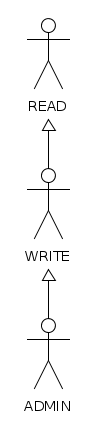
\includegraphics[width=0.05\textwidth]{imaxes/actores.png}
  \caption{Actores del sistema}
  \label{fig:actores}
\end{figure}

El actor ADMIN representa a los usuarios de la aplicación que tienen
acceso completo a todas las funciones, incluyendo la gestión de usuarios.

Los actores  READ y  WRITE representa a cualquier usuario con un perfil READ o WRITE que haya sido dado de alta previamente por un actor ADMIN, que representa a cualquier usuario con perfil ADMIN, y disponga de un nombre de usuario y una contraseña.



\subsection{Casos de uso}
\label{sub:casos-uso}


Todos los usuarios comparten los casos de uso de acceso y los relativos a la consulta de las entidades del sistema. El actor WRITE amplía esos casos de uso con funcionalidades de creación, modificación y borrado de entidades y por último el actor ADMIN amplía esos casos de uso con el caso de uso de administración de usuarios. Las siguientes figuras (figura \ref{fig:cu-acceso}, figura \ref{fig:cu-read-write}, figura \ref{fig:cu-admin} de las páginas \ref{fig:cu-acceso},\ref{fig:cu-read-write},\ref{fig:cu-admin}) muestran una visión de alto nivel de los distintos casos de uso definidos en el sistema. Dichos casos de uso se analizan con más detalle en los siguientes apartados.


\begin{figure}[H]
  \centering
  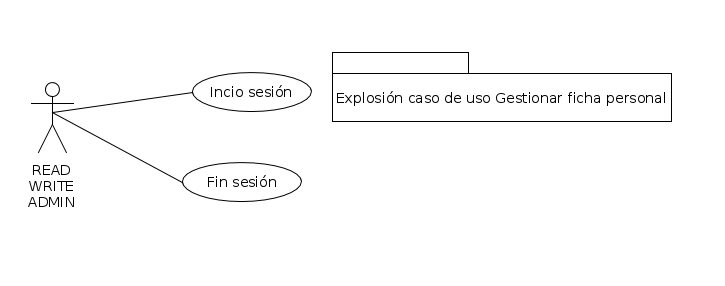
\includegraphics[width=0.50\textwidth]{imaxes/cu_acceso.png}
  \caption{Caso de uso del acceso al sistema - Actores READ, WRITE y ADMIN}
  \label{fig:cu-acceso}
\end{figure}



\begin{figure}[H]
  \centering
  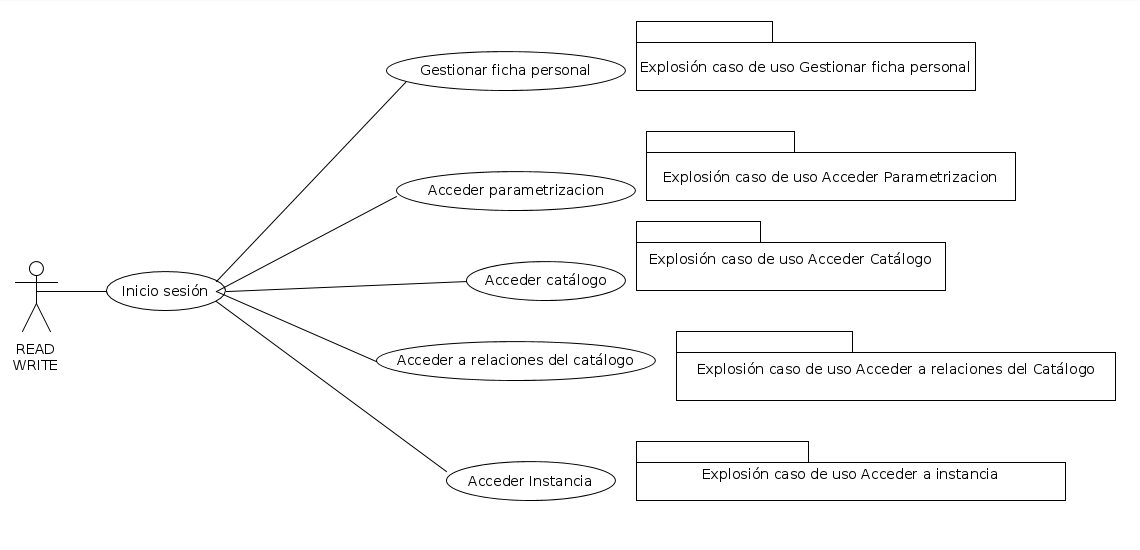
\includegraphics[width=0.50\textwidth]{imaxes/cu-read-write.png}
  \caption{Casos de uso de los actores READ, WRITE}
  \label{fig:cu-read-write}
\end{figure}


\begin{figure}[H]
  \centering
  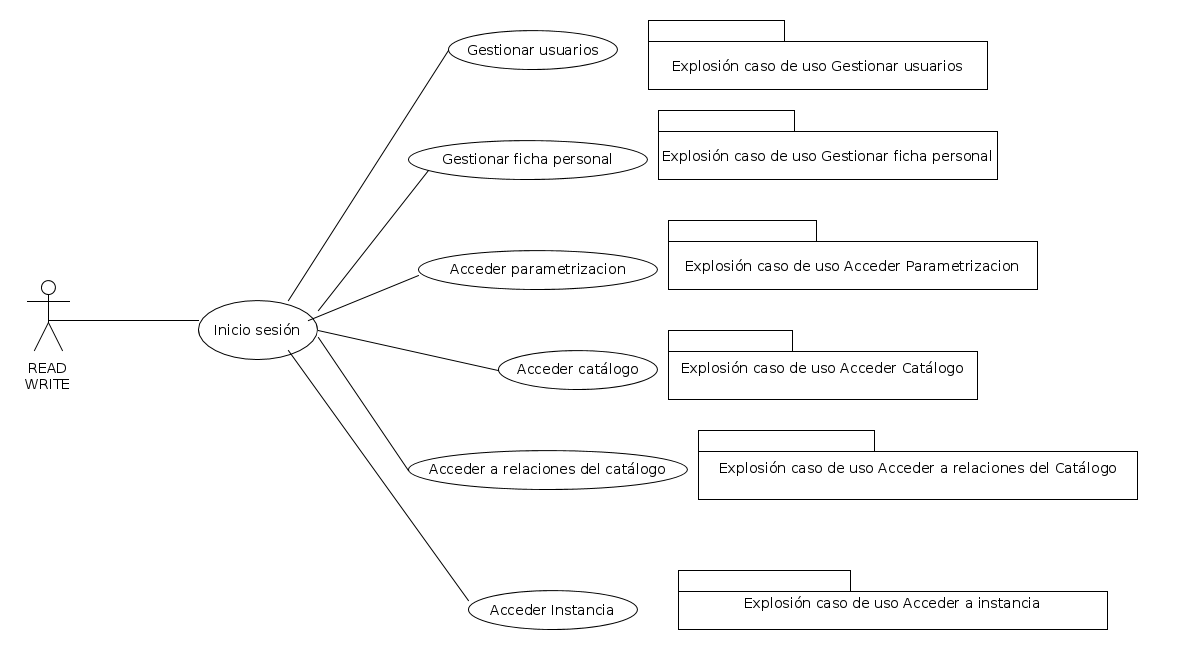
\includegraphics[width=0.50\textwidth]{imaxes/cu-admin.png}
  \caption{Casos de uso del actor ADMIN}
  \label{fig:cu-admin}
\end{figure}



A continuación se muestra un caso de uso destacable que representa
aspecto centrales de la aplicación.La definición completa de casos de uso se encuentra en el apéndice \ref{chap:ref-tecnica}. 

Se trata de los casos de uso CU-05 (tabla \ref{tab:cu-editar-historico}, página \pageref{tab:cu-editar-historico}), CU-06 (tabla \ref{tab:cu-cancelar-historico}, página \pageref{tab:cu-cancelar-historico}), CU-07 (tabla \ref{tab:cu-anhadir-historico-elemento}, página \pageref{tab:cu-anhadir-historico-elemento}) y CU-09 (tabla \ref{tab:cu-borrar-historico-elemento} página \pageref{tab:cu-borrar-historico-elemento}, que hacen referencia a la modificación de un registro de histórico de una entidad con histórico de registros (como pudiera ser un tipo de cuota). A estos casos de uso pueden acceder los actores WRITE y ADMIN a través del correspondiente caso de uso de listado de la entidad a tratar y seleccionando el correspondiente registro de histórico a modificar.

Para este tipo de entidades con registro de histórico es fundamental que exista una consecución temporal de los mismos. No puede haber registros de histórico que se solapen para una misma instacia de una entidad, ni tampoco \textit{huecos} en la línea temporal del ciclo de vida de la misma. Por lo tanto se debe revisar que los cambios producidos en las fechas de una entidad con registro de histórico sean coherentes con lo almacenado en el sistema, actualizando fechas de registros anteriores y/o posteriores en caso de ser necesario, para \textit{acortarlos} o \textit{alargarlos} según sea el caso.


\begin{table} [H]
    \centering
    \rowcolors{2}{white}{white}
    \setlength{\leftmargini}{0.4cm}
	\resizebox{14cm}{!} { % evita que la tabla sobresalga de la p\'agina, ajustando tama\'no de letra y grosor de l\'ineas
    \begin{tabular}{| m{3cm} | m{11cm} |}   
    \hline
	  \textbf{CU-05} & \textbf{Editar registro de histórico del elemento seleccionado} \\\hline
	  \textbf{Descripción} & Editar registro de histórico del elemento seleccionado. \\\hline
	  \textbf{Actores} & WRITE y ADMIN. \\\hline
	  \textbf{Precondiciones} & El usuario con perfil WRITE o ADMIN ha pulsado el botón editar para el registro de histórico para el elemento seleccionado. \\\hline
	  \textbf{Postcondiciones} & Se modifica el registro de histórico elemento del listado de la entidad  y, si es necesario, se modifican las fechas de los regisros registros anterior y posterior para que sean consecutivos. \\\hline
	  \textbf{Flujo básico} & 
		\begin{enumerate}
	  	\item El sistema muestra los campos editables del registro seleccionado y dos botones: guardar y cancelar.
        \item El usuario modifica los campos deseados sobre el registro. Si el estado del registro cambia al estado cancelado se dispara el caso de uso \ref{tab:cu-cancelar-historico} (página \pageref{tab:cu-cancelar-historico}).
			\begin{enumerate}	
			   \item El usuario pulsa el botón de guardar. El sistema comprueba que los campos obligatorios han sido completados y que los datos tienen el formato correcto. Realiza las modificaciones pertinentes en los registros de histórico anterior y posterior del elemento seleccionado, de forma que todos los registros de histórico sean correlativos. Se guardan los datos de fecha de creación y nombre de usuario tanto para el nuevo registro de histórico como para los registros adyacentes modificados. Se termina la edición del registro. Se informa al usuario que el registro ha sido modificado y se actualiza el listado de la entidad con las modificaciones realizadas.
			   \begin{enumerate}	
			   \item  \textit{\textbf{Flujo alternativo:} Si no se cubre algún campo obligatorio o se produce algún error de validación el sistema informa del error.}
			   \end{enumerate}
			   \item El usuario pulsa el botón cancelar. Se termina la edición del registro y se descartan los posibles cambios.
			\end{enumerate}
	  \item Finaliza el caso de uso.
	  \end{enumerate} 	  	  
	  \\\hline
    \end{tabular}
    } % end /resizebox
    \caption{CU-05 Editar histórico de elemento seleccionado}
    \label{tab:cu-editar-historico}
\end{table}


\begin{table} [H]
    \centering
    \rowcolors{2}{white}{white}
    \setlength{\leftmargini}{0.4cm}
	\resizebox{14cm}{!} { % evita que la tabla sobresalga de la p\'agina, ajustando tama\'no de letra y grosor de l\'ineas
    \begin{tabular}{| m{3cm} | m{11cm} |}   
    \hline
	  \textbf{CU-06} & \textbf{Cancelar el registro de histórico del elemento seleccionado} \\\hline
	  \textbf{Descripción} & Cancelar el registro de histórico del elemento seleccionado. \\\hline
	  \textbf{Actores} & WRITE y ADMIN. \\\hline
	  \textbf{Precondiciones} & El usuario con perfil WRITE o ADMIN ha seleccionado el estado cancelado para el registro de histórico que está modificando. \\\hline
	  \textbf{Postcondiciones} & Se propaga el estado de cancelado para todos los registros de histórico posteriores al registro seleccionado. \\\hline
	  \textbf{Flujo básico} & 
		\begin{enumerate}
	  	\item Se muestra un cuadro de diálogo solicitando propagar el estado cancelado para los registros posteriores al registro de histórico seleccionado.
        \item 
			\begin{enumerate}	
			   \item El usuario pulsa el botón de aceptar. El sistema propaga el nuevo estado al resto de registros de históricos posteriores al registro de histórico seleccionado. Se cierra el cuadro de diálogo.
			   \item El usuario pulsa el botón cancelar. Se cierra el cuadro de diálogo y se descarta el cambio de estado.
			\end{enumerate}
	  \item Finaliza el caso de uso.
	  \end{enumerate} 	  	  
	  \\\hline
    \end{tabular}
    } % end /resizebox
    \caption{CU-06 Cancelar el registro de histórico del elemento seleccionado}
    \label{tab:cu-cancelar-historico}
\end{table}


\begin{table} [H]
    \centering
    \rowcolors{2}{white}{white}    
    \setlength{\leftmargini}{0.4cm}
	\resizebox{14cm}{!} { % evita que la tabla sobresalga de la p\'agina, ajustando tama\'no de letra y grosor de l\'ineas
    \begin{tabular}{| m{3cm} | m{11cm} |}   
    \hline
	  \textbf{CU-07} & \textbf{Añadir registro de histórico del elemento seleccionado} \\\hline
	  \textbf{Descripción} & Añadir registro de histórico del elemento seleccionado. \\\hline
	  \textbf{Actores} & WRITE y ADMIN. \\\hline
	  \textbf{Precondiciones} & El usuario con perfil WRITE o ADMIN ha pulsado el botón añadir registro de histórico para el elemento seleccionado. \\\hline
	  \textbf{Postcondiciones} & Se añade un nuevo registro de histórico  comprendido entre el elemento seleccionado del listado de la entidad y el siguiente elemento de la lista, o a continuación del elemento seleccionado si no hay más elementos en la lista, modificando las fechas de dichos regisros para que sean consecutivos. \\\hline
	  \textbf{Flujo básico} & 
		\begin{enumerate}
	  	\item El sistema muestra un formulario con una copia del registro de histórico del elemento seleccionado con los campos susceptibles de modificar habilitados. El usuario modificará las fechas de inicio y/o fin del registro, así como el resto de campos que considere oportuno. 
			\begin{enumerate}	
			   \item El usuario pulsa el botón de guardar. El sistema comprueba que los campos obligatorios han sido completados y que los datos tienen el formato correcto. Evalúa las fechas de inicio y fin y realiza las modificaciones pertinentes sobre los histórico anterior y posterior del elemento seleccionado o sólo del anterior en caso de que no hubiera más registros, de forma que todos los registros de histórico sean correlativos. Se guardan los datos de fecha de creación y nombre de usuario para el nuevo registro de histórico, así como los de fecha de modificación y usuario para los registros de histórico adyacentes modificados. Se termina la edición del registro. Se informa al usuario que el elemento ha sido añadido. Se añade el registro al listado de la entidad y se actualiza con las modificaciones realizadas.
			   \begin{enumerate}	
			   \item  \textit{\textbf{Flujo alternativo:} Si no se cubre algún campo obligatorio o se produce algún error de validación el sistema informa del error.}
			   \end{enumerate}
			   \item El usuario pulsa el botón cancelar. Se vuelve al caso de uso inicial \ref{tab:cu-listar-parametrización} (\pageref{tab:cu-listar-parametrización}).
			\end{enumerate}
	  \item Finaliza el caso de uso.
	  \end{enumerate} 	  	  
	  \\\hline
    \end{tabular}
    } % end /resizebox
    \caption{CU-07 Añadir histórico de elemento seleccionado}
    \label{tab:cu-anhadir-historico-elemento}
\end{table}




\begin{table} [H]
    \centering
    \rowcolors{2}{white}{white}
    \setlength{\leftmargini}{0.4cm}
	\resizebox{14cm}{!} { % evita que la tabla sobresalga de la p\'agina, ajustando tama\'no de letra y grosor de l\'ineas
    \begin{tabular}{| m{3cm} | m{11cm} |}   
    \hline
	  \textbf{CU-09} & \textbf{Borrar histórico del elemento seleccionado} \\\hline
	  \textbf{Descripción} & Borrar histórico elemento seleccionado. \\\hline
	  \textbf{Actores} & WRITE y ADMIN. \\\hline
	  \textbf{Precondiciones} & El usuario con perfil WRITE o ADMIN ha pulsado el botón de borrar para el registro de histórico del elemento selecconado. \\\hline
	  \textbf{Postcondiciones} & Se elimina el registro de histórico del elemento seleccionado, modificando las fechas de los regisros anterior y/o posterior para que sean consecutivos. \\\hline
	  \textbf{Flujo básico} & 
		\begin{enumerate}
	  	\item El sistema muestra un cuadro de diálogo solicitando confirmación de borrado del registro de histórico del elemento seleccionado con dos botones: aceptar y cancelar.
		\item 
			\begin{enumerate}	
			   \item El usuario pulsa el botón de aceptar. El sistema elimina del el registro de histórico del elemento seleccionado y realiza las modificaciones pertinentes en los registros de histórico anterior y posterior del elemento seleccionado, de forma que todos los registros de histórico sean correlativos. Se informa al usuario que el elemento ha sido borrado. Se elimina el elemento del listado de la entidad  y se actualiza con las modificaciones realizadas. Se cierra el cuadro de diálogo.
			   \begin{enumerate}	
			   \item  \textit{\textbf{Flujo alternativo:} Si se produce algún error el sistema informa del error.}
			   \end{enumerate}
			   \item El usuario pulsa el botón cancelar. Se vuelve al caso de uso inicial \ref{tab:cu-listar-parametrización} (\pageref{tab:cu-listar-parametrización}).
			\end{enumerate}
	  \item Finaliza el caso de uso.
	  \end{enumerate} 	  	  
	  \\\hline
    \end{tabular}
    } % end /resizebox
    \caption{CU-09 Borrar histórico del elemento seleccionado}
    \label{tab:cu-borrar-historico-elemento}
\end{table}




\section{Diseño}
\label{sec:disenho}

En esta sección describiremos los distintos elementos usados para el diseño de la aplicación.


\subsection{Arquitectura en tres niveles}
\label{sub:arquitectura3niveles}

Para el desarrollo de este proyecto se ha optado por el patrón de arquitectura \acrlong{mvc} que presenta una arquitectura que separa las aplicaciones en tres niveles \footnote{Aunque está comunmente aceptado capa como sinónimo de nivel, no significan lo mismo. Una \textit{\textbf{capa}} se refiere a una \textit{división funcional del software}, pero un \textit{\textbf{nivel}} se refiere a una \textit{división funcional del software que se ejecuta en una infraestructura separada}  de las otras divisiones, por lo que las capas no pueden ofrecer los mismos beneficios que los niveles} de informática lógica y física: la interfaz de usuario, el nivel donde se procesan los datos y el nivel donde se almacenan y gestionan esos datos ~\cite{ibmMVC} (figura \ref{fig:arquitectura-3-niveles}, página \pageref{fig:arquitectura-3-niveles}):

\paragraph{Nivel de presentación} es la interfaz de usuario, donde el usuario final interactúa con la aplicación. Este primer nivel puede ejecutarse en una navegador web como una aplicación de escritorio o una \acrshort{gui}.

\paragraph{Nivel de aplicación} también conocido como el nivel lógico o medio, es el núcleo de la aplicación. Se procesa la información recogida en el nivel de presantación. En ocasiones este procesado de información se realiza junto con otra información en el nivel de datos a través de lo que se conoce como  lógica empresarial: un conjunto específico de reglas empresariales. Este nivel también puede añadir, suprimir o modificar datos en el nivel de datos. Se comunica con el nivel de datos mediante llamadas a las distintas \acrshort{api}. 

\paragraph{Nivel de datos} también denominado nivel de base de datos, de acceso a datos o backend, es donde se almacena y gestiona la información procesada por la aplicación. Puede ser un sistema de gestión de base de datos relacional (PostgreSQL, MySQL, Oracle,\dots) o en un servidor de bases de datos NoSQL (MongoDB, Cassandra,\dots). 


En una aplicación de tres niveles, toda la comunicación pasa por el nivel de aplicación. Los niveles de presentación y de datos no pueden comunicarse directamente entre sí.

\begin{figure}[H]
  \centering
  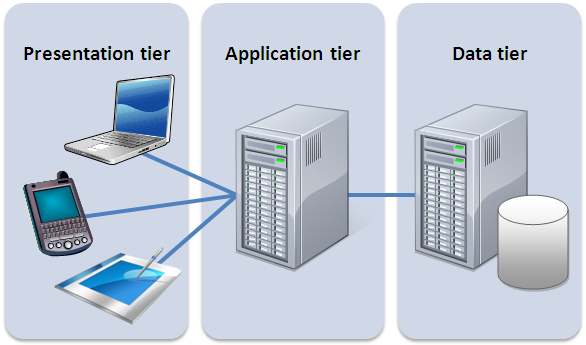
\includegraphics[width=0.50\textwidth]{imaxes/arquitectura-3-niveles.png}
  \caption{Arquitectura en tres niveles}
  \label{fig:arquitectura-3-niveles}
\end{figure}


La arquitectura de tres niveles aporta múltiples ventajas~\cite{ibmMVC}:

\begin{itemize}
\item Desarrollo más rápido: debido a que cada nivel puede ser desarrollado simultáneamente por diferentes equipos, una empresa puede llevar su aplicación al mercado más rápido y los programadores pueden utilizar los mejores y más recientes lenguajes y herramientas para cada nivel.
\item Escalabilidad mejorada: cualquier nivel se puede escalar independientemente de los demás según sea necesario.
\item Confiabilidad mejorada: es menos probable que una interrupción en un nivel afecte la disponibilidad o el rendimiento de los otros niveles.
\item Seguridad mejorada: debido a que los niveles de presentación y de datos no se pueden comunicar directamente entre sí, un nivel de aplicación bien diseñado puede funcionar como una especie de firewall interno, lo que impide ataques de inyecciones SQL y otras vulnerabilidades maliciosas.
\end{itemize}


\subsection{Patrones utilizados}
\label{sub:patrones}

A continuación se listan algunos de los patrones utilizados en el diseño de la herramienta presentada.



\paragraph{Patrón modelo vista controlador}
El framework \acrshort{jsf} se basa en el patrón \acrlong{mvc}.

Aunque el patrón \acrshort{mvc} comparte con la arquitectura de tres niveles la visión de la apliación en 3 áreas separadas, difiere en la forma de entender la comunicación entre ellas: en el patrón de modelo vista controlador las distintas capas se comunican de forma triangular, dos a dos, mientras que en la arquitectura de tres niveles toda comunicación pasa por el nivel de aplicación.


\begin{itemize}
\item Capa de persistencia: Recibe solicitudes de almacenamiento o recuperación de información por parte de la capa de negocio, es decir, es la encargada de cargar y modificar la información guardada en el servidor de base de datos. Se encarga de convertir los datos de los registros de la base de datos a objetos manejables por Jakarta EE, para lo que cuenta con un mecanismo de conversión de datos relacionales a objetos. 
\item Capa de negocio: Se encarga de las reglas del negocio que resuelve o satisface las necesidades de un dominio en un negocio particular. En este nivel se encuentra en el servidor de aplicaciones. Los componentes de este nivel interactúan con el nivel de persistencia y suelen implementarse como componentes EJB.
\item Nivel de presentación: Se encarga de interactuar con el usuario final. Contiene la lógica de presentación que se emplea para generar una respuesta al cliente y sus operaciones son soportadas por el contenedor web que es el encargado de dar un acceso visual al sistema a través de una interfaz de usuario como la web a través de un navegador. Esta capa utiliza la capa de negocio para realizar ciertas operaciones.
\end{itemize}


\begin{figure}[H]
  \centering
  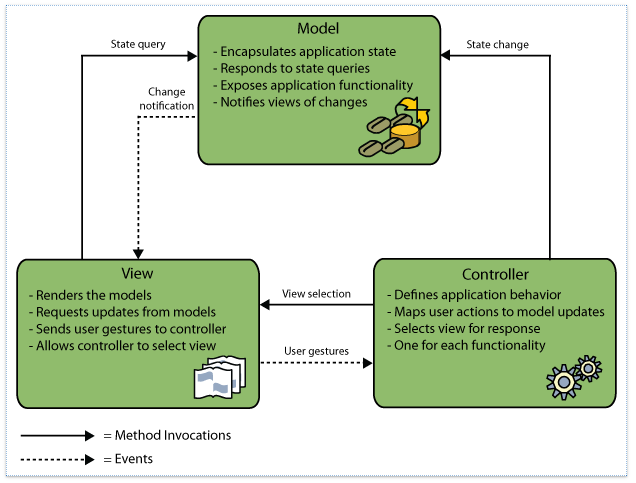
\includegraphics[width=0.50\textwidth]{imaxes/mvc-patron.png}
  \caption{Patron MVC}
  \label{fig:patron-mvc}
\end{figure}




    
\paragraph{Composite View}
El sistema de plantillas de JSF se basa en el patrón de diseño Composite View,
lo que significa que las secciones de una página o incluso las propias páginas pueden ser reutilizadas por otras páginas.
Se han utilizado plantillas en el diseño de la ventana principal de la aplicación, la barra de herramientas de la aplicación que contiene el acceso al menú y a la información del usuario, así como la información de la vista actual.


\paragraph{DTO - Data Transfer Object}
Se utiliza este patrón para reducir el número de llamadas a métodos mediante el uso de objetos que transportan datos entre procesos. También permite la encapsulación de la lógica de la serialización (el mecanismo que traduce la estructura del objeto y los datos a un formato específico que se puede almacenar y transferir) proporcionando un único punto de cambio en los matices de serialización.

Los objetos de este patrón generalmente se crean como \acrlong{pojo}. Se trata de estructuras de datos planas que no contienen lógica de negocio, sólo  almacenamiento, accesorios y, finalmente, métodos relacionados con la serialización o el análisis.


\paragraph{DAO - Data Access Object}
Se usa este patrón para abstraer y encapsular todos los accesos al almacén de datos persistente, gestionando la conexión con el origen de datos para obtener y almacenar los datos. 
Este patrón ha sido utilizado en la herramienta para insertar, modificar y borrar los distintos datos de la base de datos.



